En este capítulo, se observan las diferentes pantallas que responden a las consultas realizadas a la MIB de Linux y de Windows y que de igual manera, muestra el segundo punto de la práctica que se refiere a la utilización del comando snmpget y algunos otros.
\section{Cuestionario}
\begin{enumerate}
\cfinput{Cuestionario/preguntasMarcela}
\cfinput{Cuestionario/preguntasRosa}
\cfinput{Cuestionario/preguntasSamuel}


\item ¿El agente ha recibido mensajes TCP? ¿Cuántos?\\
El resultado para Linux se muestra en la figura \ref{image:tcpget} y en la figura \ref{image:tcpnext}, en la primera se muestra la ejecución con el comando snmpget y en la segunda se muestra el resultado que el comando snmpgetnext arroja, que es el valor del índice siguiente al solicitado en la consola.

\FloatBarrier
\begin{figure}[htbp!]
		\centering
	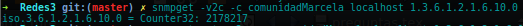
\includegraphics[width=.9 \textwidth]{images/tcpget}
		\caption{Número de mensajes TCP recibidos en Linux con comando snmpget.}		\label{image:tcpget}
\end{figure}
\FloatBarrier


\FloatBarrier
\begin{figure}[htbp!]
		\centering
	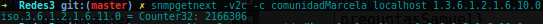
\includegraphics[width=.9 \textwidth]{images/tcpnext}
		\caption{Número de mensajes TCP recibidos en Linux con comando snmpgetnext.}		\label{image:tcpnext}
\end{figure}
\FloatBarrier

Por otro lado, el resultado para Windows se muestra en las figuras \ref{image:tcpgetW} y en la figura \ref{image:tcpnextW}, mostradas a continuación:
\FloatBarrier
\begin{figure}[htbp!]
		\centering
	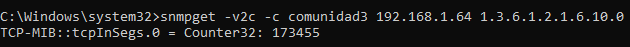
\includegraphics[width=.9 \textwidth]{images/tcpgetW}
		\caption{Número de mensajes TCP recibidos en Windows con comando snmpget.}		\label{image:tcpgetW}
\end{figure}
\FloatBarrier


\FloatBarrier
\begin{figure}[htbp!]
		\centering
	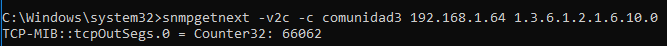
\includegraphics[width=.9 \textwidth]{images/tcpnextW}
		\caption{Número de mensajes TCP recibidos en Windows con comando snmpgetnext.}		\label{image:tcpnextW}
\end{figure}
\FloatBarrier


\item ¿Cuántos mensajes EGP ha recibido el agente?

Debido a que el grupo  \textbf{EGP} está asociado a la comunicació de la interconexión de redes externas. El alcance de la implementación se  \textbf{SNMP} se limita a equipos de la misma red, por esa razón no se encuentran mensajes EGP en ambos agentes, a continuación se muestran los resultados de la consulta egpInMsgs.


\textbf{Consulta SNMP: egpInMsgs Windows OID: 1.3.6.1.2.1.8.1.0 (figura \ref{image:11-W})}
\FloatBarrier
\begin{figure}[htbp!]
		\centering
	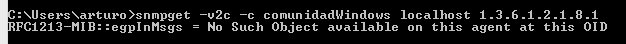
\includegraphics[width=.9 \textwidth]{images/11-W}
		\caption{S.O Windows no tiene mensajes EGP}		\label{image:11-W}
\end{figure}
\FloatBarrier


\textbf{Consulta SNMP: egpInMsgs Centos OID: 1.3.6.1.2.1.8.1.0 (figura \ref{image:11-C})}
\FloatBarrier
\begin{figure}[htbp!]
		\centering
	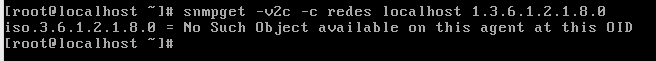
\includegraphics[width=.9 \textwidth]{images/11-C}
		\caption{S.O Centos no cuenta con mensajes EGP}		\label{image:11-C}
\end{figure}
\FloatBarrier

\item Indica el Sistema Operativo que maneja el agente.


Con el grupo System de  la MIB SNMP encontramos la información relacionada a los agentes, con la \textbf{consulta SNMP sysDescr} podemos ver la información del agente tanto a nivel Hardware como Software, los puntos más importantes de la consulta SNMP es el sistema operativo con el cual cuenta el agente y la versión, como se puede ver en la imagen  \ref{image:12-W}  muestra la descripcion del Sistema Windows y en la imagen   \ref{image:12-c}   del Sistema Operativo Linux.
 
\FloatBarrier
\begin{figure}[htbp!]
		\centering
	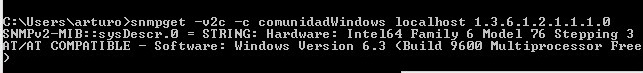
\includegraphics[width=.9 \textwidth]{images/12-W}
		\caption{Información del Sistema Operativo Windows}		\label{image:12-W}
\end{figure}
\FloatBarrier

En cuanto a la consulta SNMP realizada en Windows con el OID: 1.3.6.1.2.1.1.1.0, se muestra en la figura \ref{image:12-c}.
\FloatBarrier
\begin{figure}[htbp!]
		\centering
	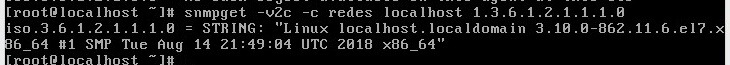
\includegraphics[width=.9 \textwidth]{images/12-c}
		\caption{Información del Sistema Operativo Centos}		\label{image:12-c}
\end{figure}
\FloatBarrier


\item Modifica el nombre del contacto o la ubicación del sistema de un agente.

Con la consulta snmpset podemos modificar el valor de un OID, esto se hace mediante el comando \textbf{snmpset versión -c comunidad localhost OID s "El nuevo valor"}. A continuación se muestran los resultados de la consulta en el Sistema Operativo Windows  \ref{image:131}  y Sistema Operativo Linux  \ref{image:13-c}



\textbf{Consulta snmpset: sysContact(4) sysUbication(6) Windows (figura   \ref{image:131}) y   (figura  \ref{image:132})}
\FloatBarrier
\begin{figure}[htbp!]
		\centering
	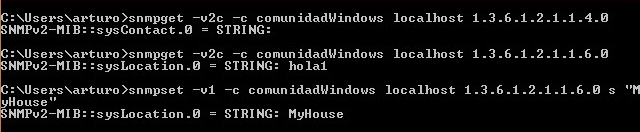
\includegraphics[width=.9 \textwidth]{images/131}
		\caption{valores de sysContact y sysUbcation, se cambio la ubicación del agente a "MyHouse"}		\label{image:131}
\end{figure}
\begin{figure}[htbp!]
		\centering
	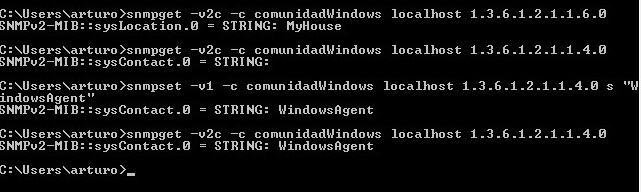
\includegraphics[width=.9 \textwidth]{images/132}
		\caption{Se cambio el valor de sysContact "WindowsAgent" y se muestran los cambios hechos en sysContact y sysUbication}		\label{image:132}
\end{figure}
\FloatBarrier


\textbf{Consulta snmpset: sysContact(4) sysUbication(6) Centos (figura  \ref{image:13-c}) y   (figura  \ref{image:13-c1})}
\FloatBarrier
\begin{figure}[htbp!]
		\centering
	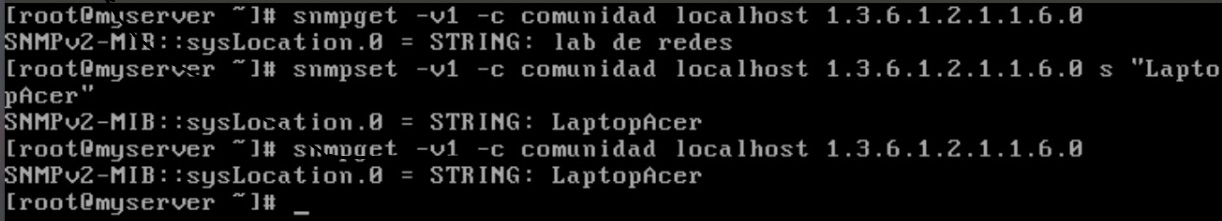
\includegraphics[width=.9 \textwidth]{images/13-c}
		\caption{Se cambio el valor de sysUbication(6) "LaptopAcer" y se muestran los cambios hechos del valor inicial al final}		\label{image:13-c}
\end{figure}
\begin{figure}[htbp!]
		\centering
	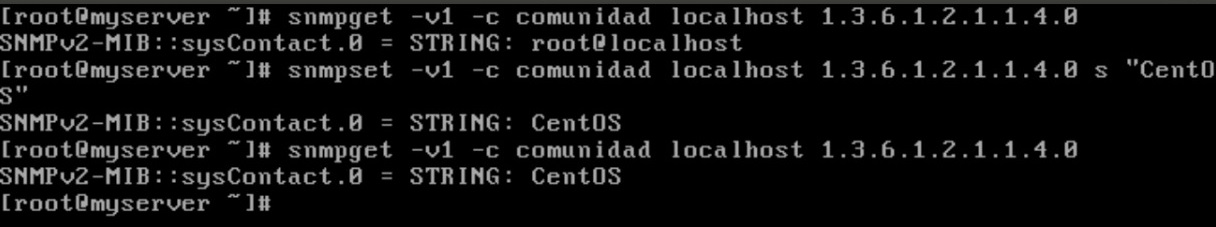
\includegraphics[width=.9 \textwidth]{images/13-c1}
		\caption{Muestra el valor de sysContact(4) y se modifica por "CentOS" finalmente muestra el cambio.}		\label{image:13-c}
\end{figure}
\FloatBarrier



\item Dibuja la MIB del agente.

Observamos en la figura \ref{image:dibujoMib}, la ejecución del comando \textbf{snmpwalk} al OID \textbf{1.3.6.1.2.1} correspondiente al objeto \textbf{mib-2}.
\FloatBarrier
\begin{figure}[htbp!]
		\centering
	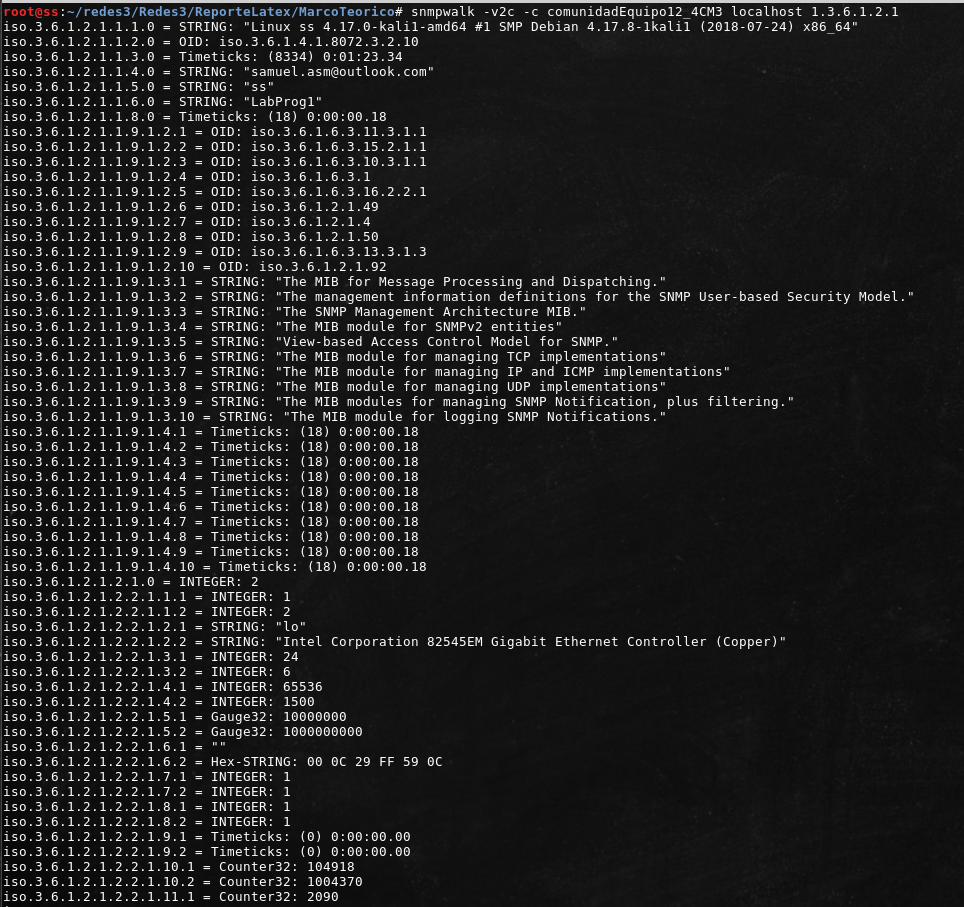
\includegraphics[width=.9 \textwidth]{images/dibujoMib}
		\caption{Dibujo de la MiB.}
\label{image:dibujoMib}
\end{figure}
\FloatBarrier
\end{enumerate}